\documentclass[
10pt,
a4paper
]{scrartcl}

\usepackage[ngerman]{babel}
\usepackage[utf8]{inputenc}
\inputencoding{utf8}
\usepackage{xcolor}
\usepackage{ulem} % underline styles
\usepackage{tikz} % for double underlines
\newcommand{\udensdash}[1]{%
    \tikz[baseline=(todotted.base)]{
        \node[inner sep=1pt,outer sep=1pt] (todotted) {#1};
        \draw[densely dashed] (todotted.south west) -- (todotted.south east);
    }%
}%

%\udensdash{\underline{PrimAndForeignKey}}

\usepackage{graphicx}
\usepackage{listings}

\lstset{language=SQL} 

\title{DBS Projekt SS2014}
\author{Jan Corsten, Frederic Prackwieser, Franz Rhee}
\date{\today}

\begin{document}

\maketitle
\tableofcontents

\section*{Einleitung}

Es soll eine Datenbank f\"{u}r die Fußball Bundesliga realisiert werden. Die Datenbank speichert Vereine, Spiele, Spieler, und Ligen. Eine Anwendung stellt vergangene Fußballergebnisse bereit. Spieler sind Vereinen zugeordnet. Vereine sind Ligen zugeordnet. Spiele finden immer zwischen einem Gastgeber und einem Gast statt.
Weiterhin wird die Datenbank für eine Data Mining Anwendung zur Ergebnisprognose genutzt.

\section{Erste Iteration}

\subsection{Aufgabenstellung}

\begin{enumerate}
  \item ERDD mit umgekehrter Chen-Min-Max-Notation in DIA erstellen
  \item Relationales Modell erstellen
  \item Datenbank mit dem Namen “bundesliga” anlegen
  \item Überführen des relationalen Modells in SQL (DDL)
  \item Erstellen der Tabellen in der Datenbank “bundesliga”
\end{enumerate}

\subsection{ERDD mit umgekehrter Chen-Min-Max-Notation}

Um das ERDD mit umgekehrter Chen-Min-Max-Notation zu erstellen, haben wir aus der Anwendungsbeschreibung fünf Entitätstypen identifiziert und jenen folgende Attribute  zugeordnet:

 \begin{itemize}
  \item \textbf{Liga}
  \begin{itemize}  
     \item Id
      \item Name
   \end{itemize}

 \item\textbf{ Verein}
  \begin{itemize}  
     \item Id
      \item Name
   \end{itemize}

\item \textbf{Spieler}
  \begin{itemize}  
     \item Id
      \item Name
     \item Trikotnummer
      \item Name
   \end{itemize}

\item \textbf{Tor}
  \begin{itemize}  
     \item Id
   \end{itemize}

\item \textbf{Spiel}
  \begin{itemize}  
     \item Id
      \item Ergebnis: ToreHeim, ToreAus
     \item Termin: Datum, Uhrzeit
      \item Spieltag
    \item Saison
   \end{itemize}
 \end{itemize}

Zwischen diesen Entitätstypen haben wir diese Beziehungen beobachtet:\\
\\
\textbf{Liga – Verein}\\
In einer Liga spielen 1 bis 25 Vereine\\
Ein Verein spielt in keiner oder einer Liga\\
\\
\textbf{Verein – Spieler}\\
Ein Verein hat 11 bis unendlich viele Spieler\\
Ein Spieler spielt in genau einem Verein\\
\\
\textbf{Verein – Spiel}\\
Ein Verein hat 1 bis 25 Spiele als Gast- und als Heimverein\\
Ein Spiel hat ein Gast- und ein Heimverein\\
\\
\textbf{Spiel – Tor}\\
Ein Spiel hat 0 bis unendlich viele Tore\\
Ein Tor wird in genau einem Spiel geschossen \\
\\
\textbf{Spieler – Tor}\\
Ein Spieler schie"st keine oder unendlich viele Tore\\
Ein Tor wird von genau einem Spieler geschossen \\ 
\\

Abbildung~\ref{fig1} bildet unsere Modellierung als ERDD mit umgekehrter Chen-Min-Max-Notation ab.

\begin{figure}[hb]
	\centering
  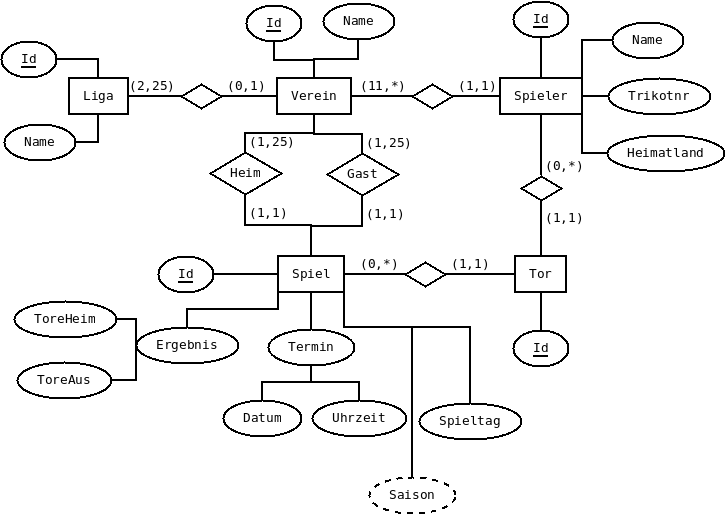
\includegraphics[scale=0.5]{bundesliga_iter1.png}
	\caption{ERDD mit umgekehrter Chen-Min-Max-Notation}
	\label{fig1}
\end{figure}

\subsection{Modifikation der Modellierung}

Wir haben festgestellt, oder vielmehr wurden wir in der ersten Iterationspräsentation darauf hingewiesen, dass obiges Modell keine hinreichende Abbildung der Anwendungsbeschreibung darstellt, da nicht alle Anfragen beantwortet werden können. Daraufhin haben wir unser Design überarbeitet und in Abbildung~\ref{fig2} ein ERRD erstellt das nun folgende Anfragen ermöglicht:

 \begin{itemize}
  \item Vereinswechsel von Spieler
  \item Welche Tore für welchen Verein
  \item Welche Trikotnummer
  \item Welcher Verein spielt wann in welcher Liga
\end{itemize}

\begin{figure}[h]
	\centering
  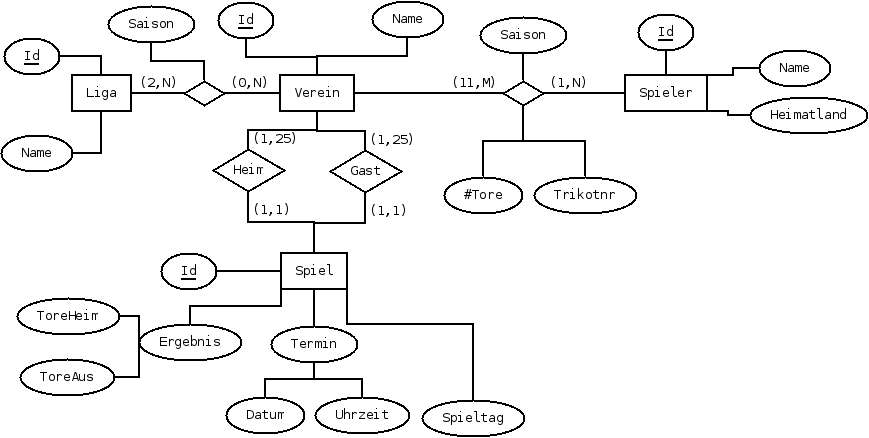
\includegraphics[scale=0.4]{bundesliga.png}
	\caption{Modifiziertes ERDD mit umgekehrter Chen-Min-Max-Notation}
	\label{fig2}
\end{figure}

\subsection{Relationales Modell }

Abbildung~\ref{fig3} zeigt das relationale Modell, welches wir aus dem überarbeiteten ERDD übersetzt haben. Es zeigt die aus dem ERDD abgelesenen Relationen und die Fremdschlüssel  Abhängigkeit dieser auf.

\begin{figure}[h]
	\centering
  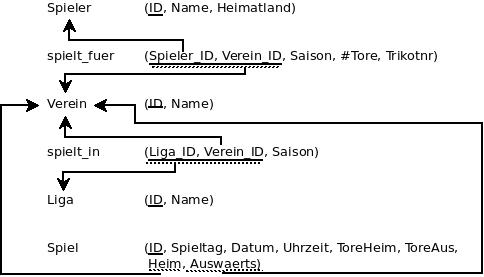
\includegraphics[scale=0.6]{relat.jpg}
	\caption{Relationales Modell }
	\label{fig3}
\end{figure}

\subsection{Erstellen der Tabellen in der Datenbank “bundesliga”}
Anhand des relationalen Modells aus Abbildung~\ref{fig3} haben wir nun mit folgenden SQL Queries die benötigten Tabellen für unsere Bundesliga Datenbank erstellt.
 
\lstinputlisting[language=Sql, firstline=29, lastline=148, frame=single]{../dbs-sql/FU_Buli_create.sql}

\subsection{Projektverlauf der ersten Iteration}

Die genauen Arbeitsanweisungen des Projekts wurden im Tutorium von Nicolas Lehmann vorgestellt. Daraufhin haben sich drei Unbekannte  zu einem Team zusammengefunden, um das Projekt in Angriff zu nehmen.\\
Für die erste Iteration haben wir uns darauf geeinigt PostgreSQL zu verwenden, und für die Erstellung der Diagramme Dia zu benutzen. Unsere Kommunikation erfolgte überwiegend per Email und für den Austausch von Daten haben wir das git  Repository https://github.com/hrhee/dbs-project-ss14/ genutzt.\\
In einem Projekttreffen vor der Präsentation der ersten Iteration, haben wir die Aufgabenstellungen zusammen diskutiert und gemeinsam Lösungen gefunden.

\subsubsection{Aufgabenaufteilung}
\begin{tabular}{ l l c }
Jan Corsten & SQL Queries &  3h \\
Frederic Prackwieser & Erstellung des ERRD in Dia  & 3h \\
Franz Rhee & Präsentation & 1h \\
\end{tabular}

\section{ Zweite Iteration}

\subsection{Aufgabenstellung}

\begin{enumerate}
  \item Datentransformation mit SQL  
  \item Datentransformation mit Java
  \item Data Mining: Einen Klassifikator lernen (Klassifikator erstellen) welcher ein kommendes Spielergebnis prognostizieren kann
\end{enumerate}

\subsection{Datentransformation mit SQL}
\lstinputlisting[language=Sql, frame=single]{../dbs-sql/FU_Buli_import.sql}

Hierzu haben wir uns erstmal entschieden von PostgreSQl auf MySQL umzusteigen, um die Datenbank der Universit"at Bayreuth, die mit MySQL erstellt wurde, leichter importieren zu k"onnen. Wir haben dann das Tool phpMyAdmin benutzt, um die Datenbank zu importieren und die Datentransformation durchzuf"uhren.

Nachdem wir unser "uberarbeitetes relationales Modell aus Abbildung \ref{fig3} auch in My{-}SQL "uberf"uhrt haben, konnten wir dann die gew"unschten Spalten aus der importierten Datenbank "`bundesliga"' ausw"ahlen und in unsere Datenbank "`mybuli"' importieren. Die entsprechenden SELECT- und IMPORT Anweisungen sind in Listing \ref{listingsql}.

\lstinputlisting[language=Sql, frame=single, caption=Datentransformation mit SQL, 
label=listingsql]{../dbs-sql/FU_Buli_import.sql}

\subsection{Datentransformation mit Java}

\subsection{Data Mining}
Als ersten Schritt haben wir uns zusammen neben den geforderten noch weitere sinnvolle Features überlegt
und uns für folgende entschieden:

 \begin{itemize}
  \item Tore der letzten 3 Spiele
  \item Gegentore der letzten 3 Spiele
  \item Anzahl Niederlagen der letzten 5 Spiele
  \item durchschnittliche Steigung der Tore der letzten 5 Spielen
  \item Ist das Spiel ein Heimspiel?
  \item Ergebnis des letzten Spiels
  \item Tore der letzten drei Heimspiele
 \end{itemize}

Abbildung~\ref{fig5} zeigt den Aufbau des Java Codes zur Erstellung der Arff-Datei.
\begin{figure}[ht]
\centering
  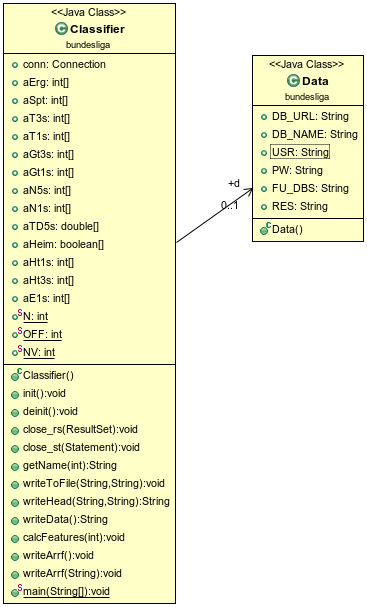
\includegraphics[scale=0.7]{Classifier.png}
\caption{Klassendiagramm: Classifier}
\label{fig5}
\end{figure}

Die Daten für die Arff-Datei werden in der Methode calcFeatures erstellt.
Für jeden Verein wird ein Datensatz mit den oben genannten Attributen nacheinender erstellt
\lstinputlisting[language=java, firstline=189, lastline=292, breaklines=true, frame=single]{../dbs-java/src/bundesliga/Classifier.java}

Und letztendlich erhielten wir folgende Ausgabe

\begin{figure}[ht1]
\centering
  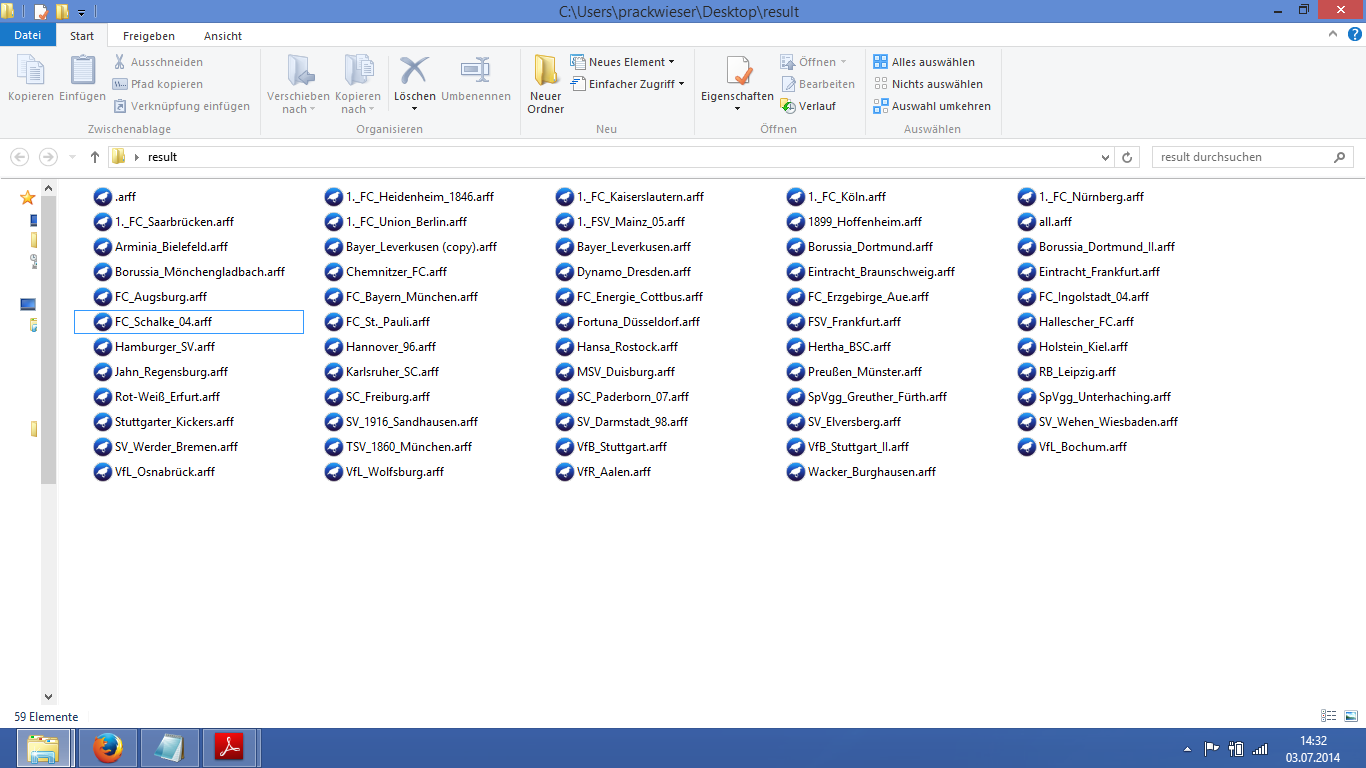
\includegraphics[scale=0.3]{Ausgabe.png}
\caption{Übersicht des Ausgegebenen Arff-Dateien}
\label{fig6}
\end{figure}

Nun mussten wir überlegen, was für eine Art von Prognose wir eigentlich anhand der Daten bekommen können.
Letztendlich gibt es die Möglichkeit anhand eines Trainingssets( z.B. die letzten 10 Spiele) die nächsten Spiele für einen Verein zu prognostizieren
und wir erhielten das folgende Ergebnis

\begin{figure}[ht2]
\centering
  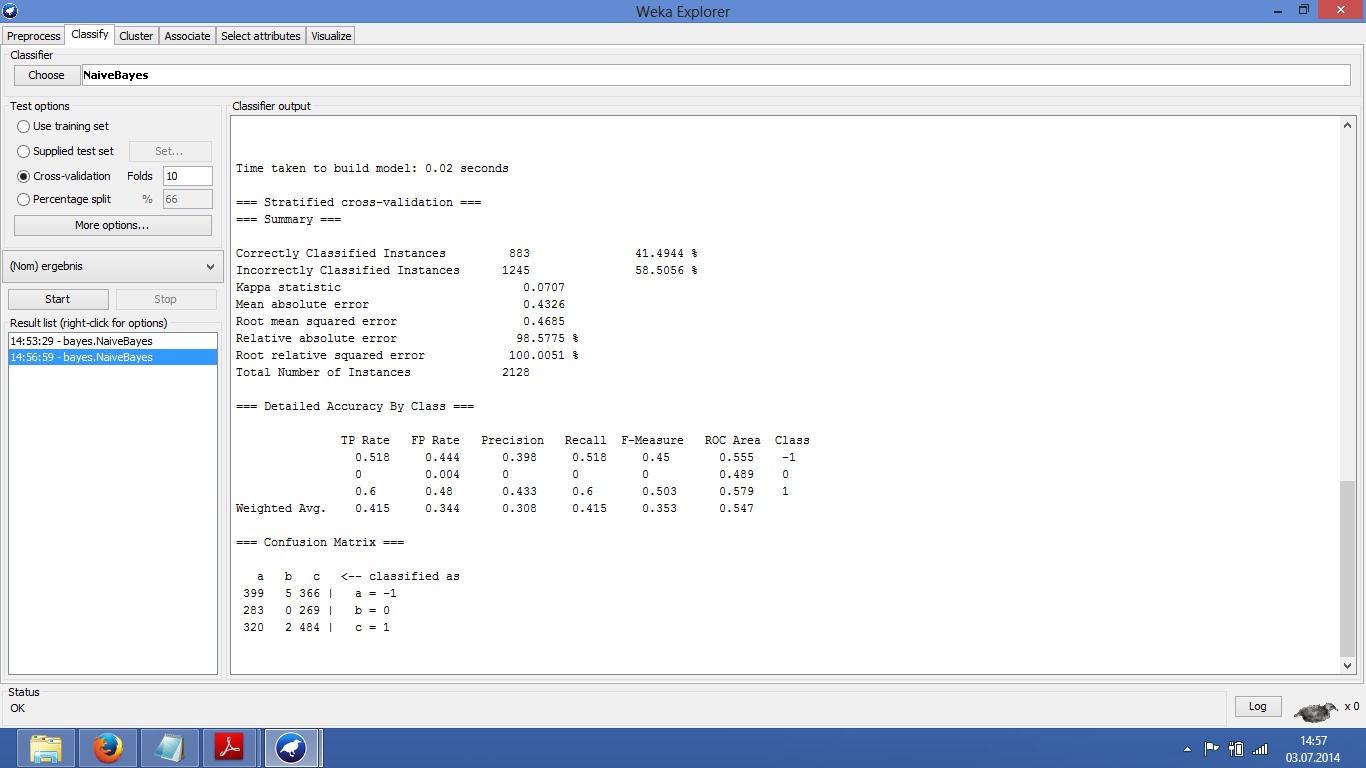
\includegraphics[scale=0.3]{Weka2.png}
\caption{Beispiel Bayern München}
\label{fig7}
\end{figure}

Ebenso kamen wir auf die Idee aus den Spielen aller Vereine die Ergebnisse kommender Spiele vorauszusagen

\begin{figure}[ht3]
\centering
  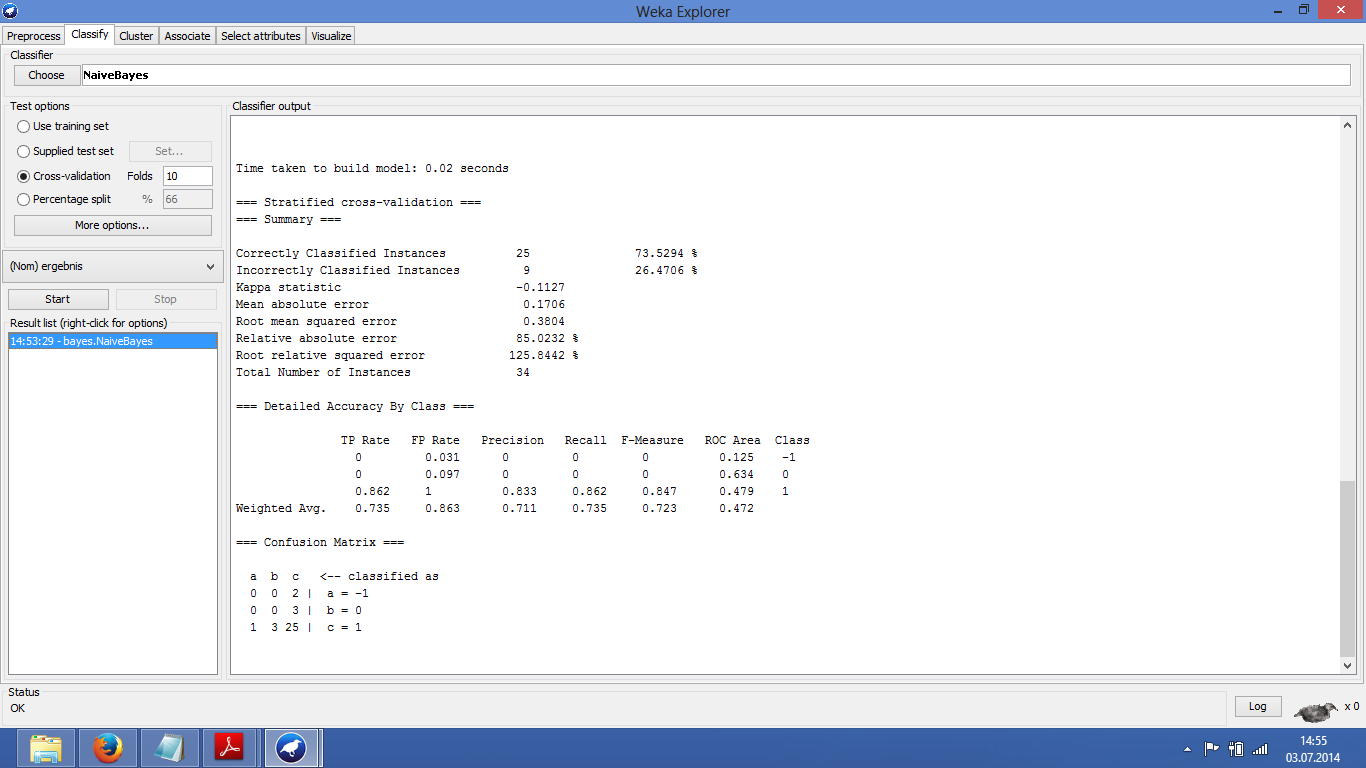
\includegraphics[scale=0.3]{Weka1.png}
\caption{Beispiel alle Spiele}
\label{fig8}
\end{figure}

Wir stellten fest, dass die Genauigkeit für einen durchschnittlichen Verein oft bei über $50\%$ liegt und manchmal sogar bei über $70\%$
und somit deutlich besser als für zufälliges Vorhersagen ist.

\subsection{Projektverlauf der zweiten Iteration}
Insgesamt waren die Arbeitsabläufe innerhalb unseres Teams ähnlich der letzten Iteration. Wir nutzten wieder das github Repository zum Austausch.


 

\subsubsection{Aufgabenaufteilung}
\begin{tabular}{ l l c }
Jan Corsten & SQL Queries, Präsentation & 5h \\
Frederic Prackwieser & Data Mining & 5h \\
Franz Rhee & Java und Weka & 10h \\
\end{tabular}

\end{document}
